
\chapter{The first ray of the Sun -- II}
\label{sec:el-primer-rayo-de-sol-ii}

\lettrine[ante=\raisebox{-1.5ex}{\Large ---},lines=2]{Y}{ou} still have to extrude the polygon---Antonia began the chapter going directly to the point.

    \begin{center}
    \begin{lstlisting}
alto_pixel = 2;
ancho_pixel = 6;
radio_semicilindro = 30;
H = radio_semicilindro+10;

module rayo_de_sol(alfa){
  D=H/tan(alfa);
  vertices=[[-alto_pixel/2,0],
            [D-alto_pixel/2,H],
            [D+alto_pixel/2,H],
            [alto_pixel/2,0]];
  linear_extrude(ancho_pixel)
    polygon(vertices);
}
 
rayo_de_sol(alfa=60);
    \end{lstlisting}
  \end{center}

  \begin{figure}[t]
    \centering
  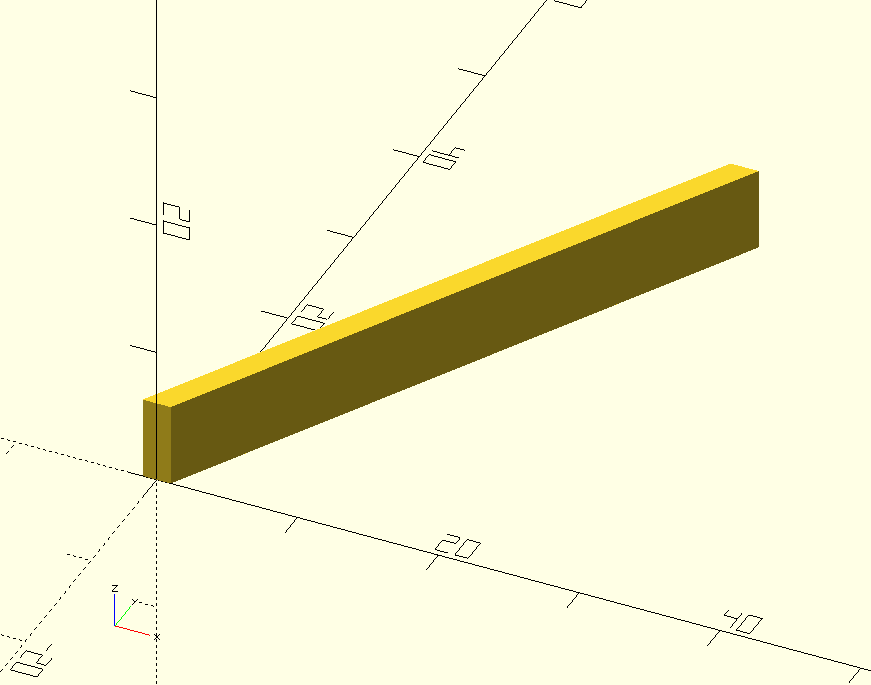
\includegraphics[width=.6\textwidth]{imagenes/rayo-extrudido-1}  
  \caption{Extruded sunbeam waiting to be rotated.}
    \label{fig:rayo-extrudido-1}
  \end{figure}
  
---And now, to rotate it!---Cecilia intervened, laughing and taking the keyboard for herself.

%    \begin{center}
\begin{lstlisting}
alto_pixel = 2;
ancho_pixel = 6;
radio_semicilindro = 30;
H = radio_semicilindro+10;

module rayo_de_sol(alfa){
  D=H/tan(alfa);
  vertices=[[-alto_pixel/2,0],
            [D-alto_pixel/2,H],
            [D+alto_pixel/2,H],
            [alto_pixel/2,0]];
  rotate([90,0,0])
    linear_extrude(ancho_pixel)
      polygon(vertices);
}
 
rayo_de_sol(alfa=60);
\end{lstlisting}
 % \end{center}

  \begin{figure}[t]
    \centering
  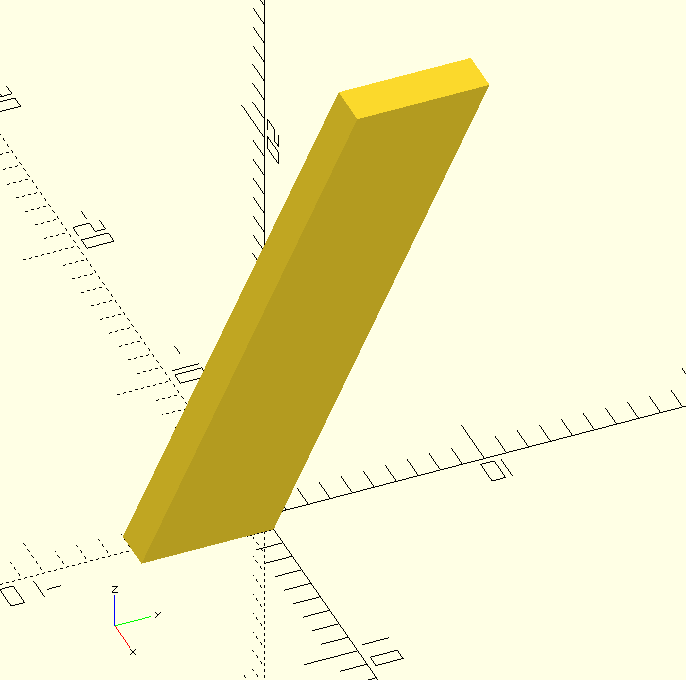
\includegraphics[width=.48\textwidth]{imagenes/rayo-extrudido-2}    
    \caption{First Sunbeam rotated by Cecilia.}
    \label{fig:rayo-extrudido-2}
  \end{figure}

Cecilia happily admired the result in the figure~\ref{fig:rayo-extrudido-2}: they were getting closer to their long-awaited digital sundial. However, one detail froze his smile: he noticed that the base of the beam was not centered at the origin, but rather shifted:

---Antonia, the ray is now on the negative  \coord{Y}: won't that be a problem? Do you think we translate it by   \texttt{ancho\_pixel/2} along that axis?

Antonia smiled, raising her eyebrows in admiration:

---Good for noticing the problem, and better for finding a solution. Actually, I don't know if it will be a problem later; In any case, it is always a good idea for modules to behave in the simplest way possible. In this case, everything seems to indicate that the most natural thing is for the base of the Sun's ray to be centered---Antonia paused, and her gaze seemed to see beyond the monitor---.
Indeed, it can be solved with a mere translation; just insert the code \lstinline!translate([0,ancho_pixel/2,0])! between lines 11 and 12 of your text. But there is another way:

\begin{lstlisting}
alto_pixel = 2;
ancho_pixel = 6;
radio_semicilindro = 30;
H = radio_semicilindro+10;

module rayo_de_sol(alfa){
  D=H/tan(alfa);
  vertices=[[-alto_pixel/2,0],
            [D-alto_pixel/2,H],
            [D+alto_pixel/2,H],
            [alto_pixel/2,0]];
  linear_extrude(ancho_pixel,center=true)
    polygon(vertices);
}
 
rayo_de_sol(alfa=60);
\end{lstlisting}

\begin{figure}[ht]
  \centering
  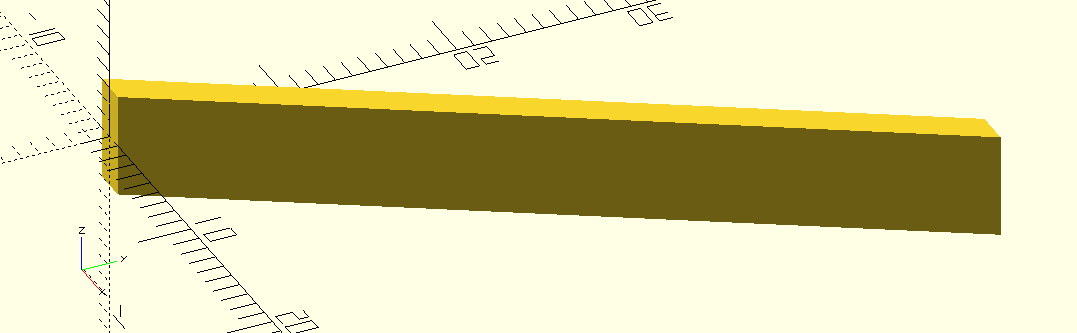
\includegraphics[width=.8\textwidth]{imagenes/rayo-extrudido-3}  
  \caption{Antonia extrudes the sunbeam polygon with the option \lstinline!center=true!.}
  \label{fig:rayo-extrudido-3}
\end{figure}


\guillemotright{}When you add the prescription \lstinline!center=true! to the transform \lstinline!linear_extrude!  (as I did on line 12), the extrusion is done centered respect to the plane \coord{XY}. Now yes, if we rotate it:

\begin{lstlisting}
alto_pixel = 2;
ancho_pixel = 6;
radio_semicilindro = 30;
H = radio_semicilindro+10;

module rayo_de_sol(alfa){
  D=H/tan(alfa);
  vertices=[[-alto_pixel/2,0],
            [D-alto_pixel/2,H],
            [D+alto_pixel/2,H],
            [alto_pixel/2,0]];
  rotate([90,0,0])
    linear_extrude(ancho_pixel,center=true)
      polygon(vertices);
}
 
rayo_de_sol(alfa=60);
\end{lstlisting}


\begin{figure}[ht]
  \centering
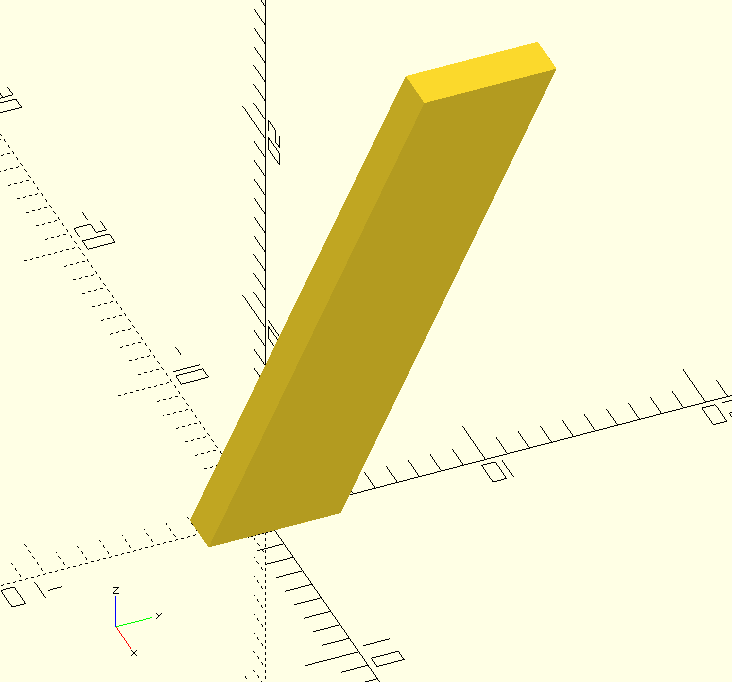
\includegraphics[width=.5\textwidth]{imagenes/rayo-extrudido-4.png}  
  \caption{Correctly centered Sunbeam.}
  \label{fig:rayo-extrudido-4}
\end{figure}

Cecilia applauded figure~\ref{fig:rayo-extrudido-4} with undisguised joy . Antonia was still concentrating with her gaze in the direction of the monitor:

---I confess that I'm not sure which of the two solutions is the best. We should take into account that our clock will be traversed by a multitude of rays, all of which must be calculated by the computer: it is always good, in those computational 'bottlenecks', to choose the most efficient algorithm --- Antonia sighed---. I don't know how the \openscad{} engine works internally. I guess the best we can do is try both
solutions, and measure how long each one takes. It is a good time to post a comment about it:

\begin{lstlisting}
module rayo_de_sol(alfa){
  D=H/tan(alfa);
  vertices=[[-alto_pixel/2,0],
            [D-alto_pixel/2,H],
            [D+alto_pixel/2,H],
            [alto_pixel/2,0]];
// TODO: medir la duracion de esta solucion
//       y la de esta otra:
// translate([0,ancho_pixel/2,0])
//       Ojo: borrar 'center=true' abajo
  rotate([90,0,0])
   linear_extrude(ancho_pixel,center=true)
    polygon(vertices);
}
\end{lstlisting}


Cecilia was too happy to dwell on those details; besides, another idea suddenly came to his attention.

\section{An alternative sunbeam?}

``Anthony!'' Cecilia exclaimed, in a vibrant tone. Let me try... Let's see... Can't you make a sunbeam like this...? ---and took the keyboard decisively, while he gave shape to his fledgling idea by writing it down.

\begin{lstlisting}
module otro_rayo_de_sol(alfa) {
  rotate([-(90-alfa),0,0])
   translate([-ancho_pixel/2,-alto_pixel/2,0])
    cube([ancho_pixel,alto_pixel,H]);  
}

otro_rayo_de_sol(alfa=60);
\end{lstlisting}


\begin{figure}[ht]
  \centering
  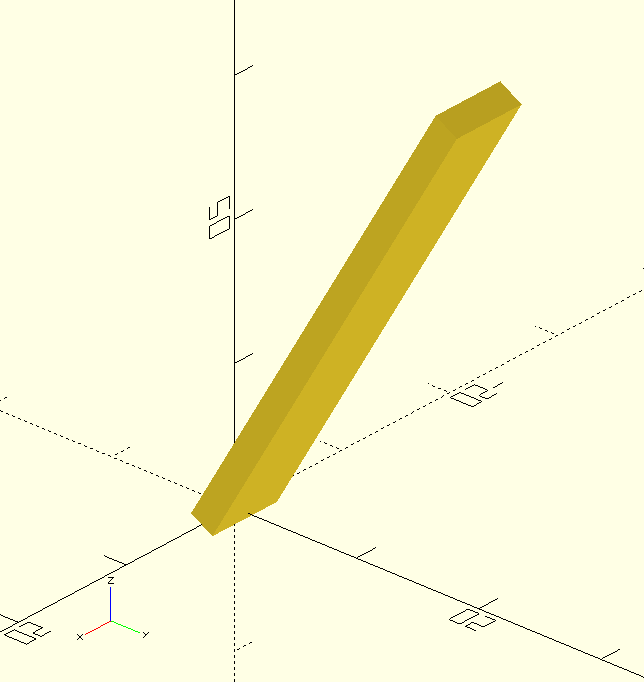
\includegraphics[width=.5\textwidth]{imagenes/otro-rayo.png}
  \caption[An alternative Sunbeam]{An alternative Sunbeam, enthusiastically proposed by Cecilia.}
  \label{fig:otro-rayo}
\end{figure}
  
Cecilia was decidedly radiant as she contemplated figure~\ref{fig:otro-rayo}. Why use a polygon, he thought, if we can use an elementary cube? He waited for a congratulation from Antonia, or at least a comment, but in vain: when he turned to look at her, he found in her only a gesture of indifferent reserve.

``I fell into that trap at first too,'' Antonia confessed . The idea of a cube seems effective, even elegant; but a disastrous detail showed me all its perversity
\footnote{Hey..! Will it be that long? (Editor's Note)}$^,$
\footnote{No: I was seized by a rhetorical attack, just. (Antonia's note)}$^,$
\footnote{Ah, ready; all good. (Editor's Note)}
 Let me show you...---Antonia began to write, under the watchful eye of her friend.


In figure~\ref{fig:otro-rayo-60} I added a floor for you to see the mark that your sunbeam, once it went through the clock, would leave on it. Don't you notice anything strange? Antonia asked.

Cecilia responded by shrugging her shoulders and raising her eyebrows.

``Yes, I understand,'' Antonia said. It's not that obvious yet. Let's see if we take a good look at it from the side, he added, producing the figure~\ref{fig:otro-rayo-60-perfil}.

``Hmmm... neither,'' Cecilia confessed.


\begin{figure}[h]
  \centering
    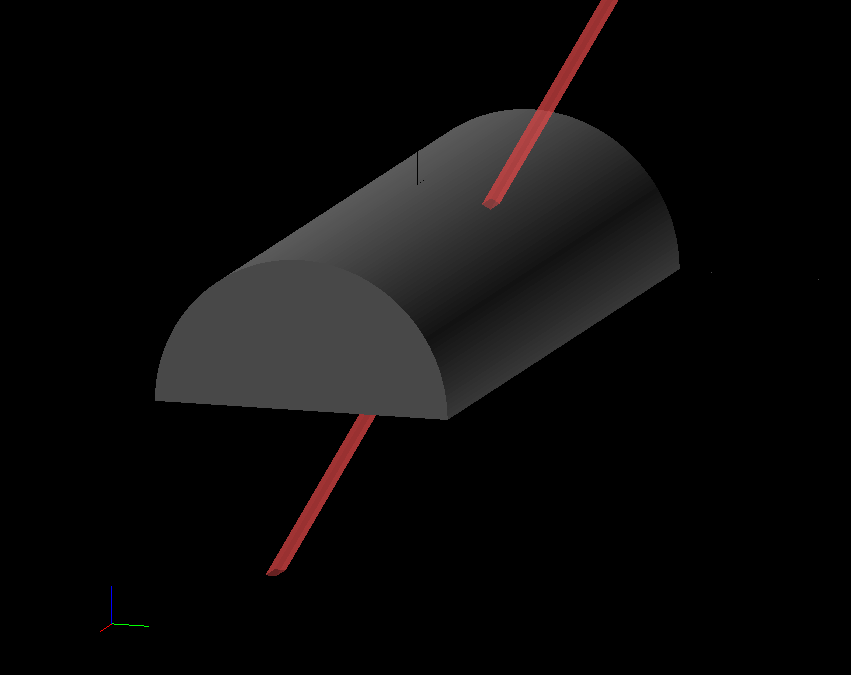
\includegraphics[width=.55\textwidth]{imagenes/otro-rayo-60.png}
    \caption[Sunbeam alternative II]{First example with which Antonia tries to dissuade Cecilia from using her alternate Sunbeam.}
\label{fig:otro-rayo-60}
\end{figure}
  

\begin{figure}[ht]
  \centering
    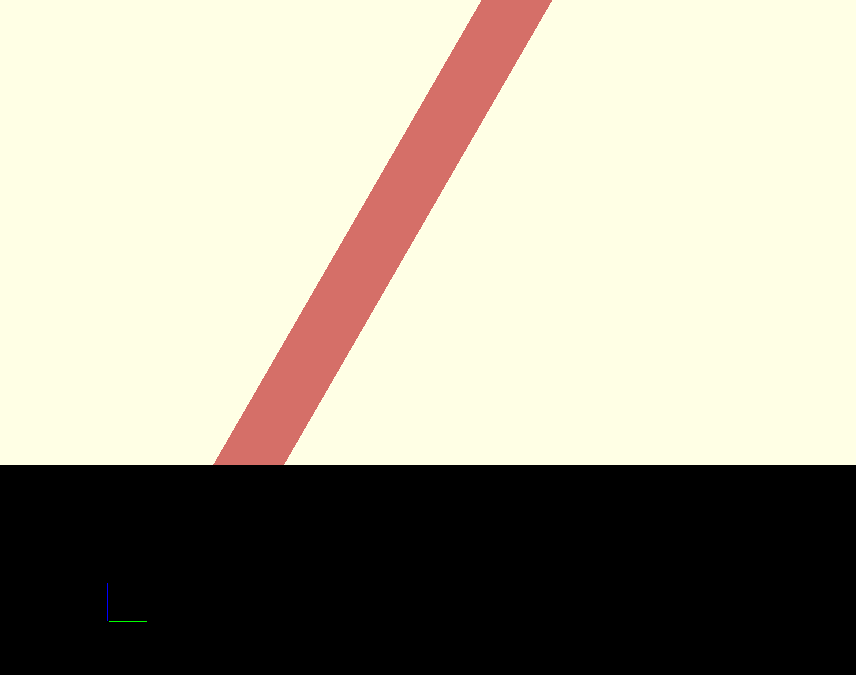
\includegraphics[width=.5\textwidth]{imagenes/otro-rayo-60-perfil}
    \caption[Sunbeam alternative  III] {Antonia continues to try to dissuade Cecilia from using her alternate Sunbeam.}
    \label{fig:otro-rayo-60-perfil}
  \end{figure}


``And with a lower angle...?'' ---Antonia tried now with figure~\ref{fig:otro-rayo-30}.

  \begin{figure}[ht]
  \centering
    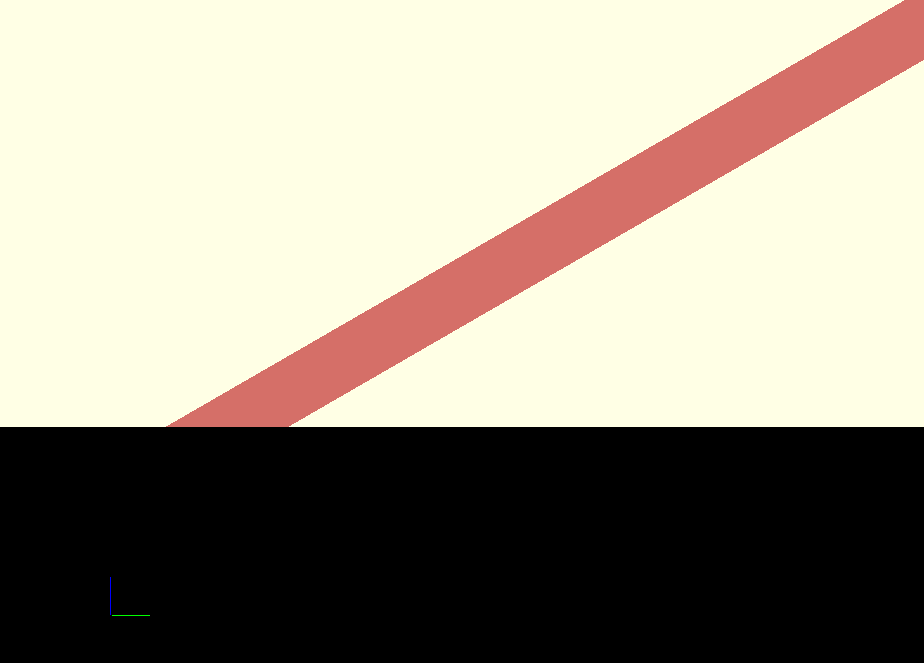
\includegraphics[width=.5\textwidth]{imagenes/otro-rayo-30}
    \caption[Sunbeam alternative  IV]{Antonia does not let up in her attempt to dissuade Cecilia from using her alternate Sunbeam.}
\label{fig:otro-rayo-30}
\end{figure}



    \begin{figure}[h!]
  \centering
    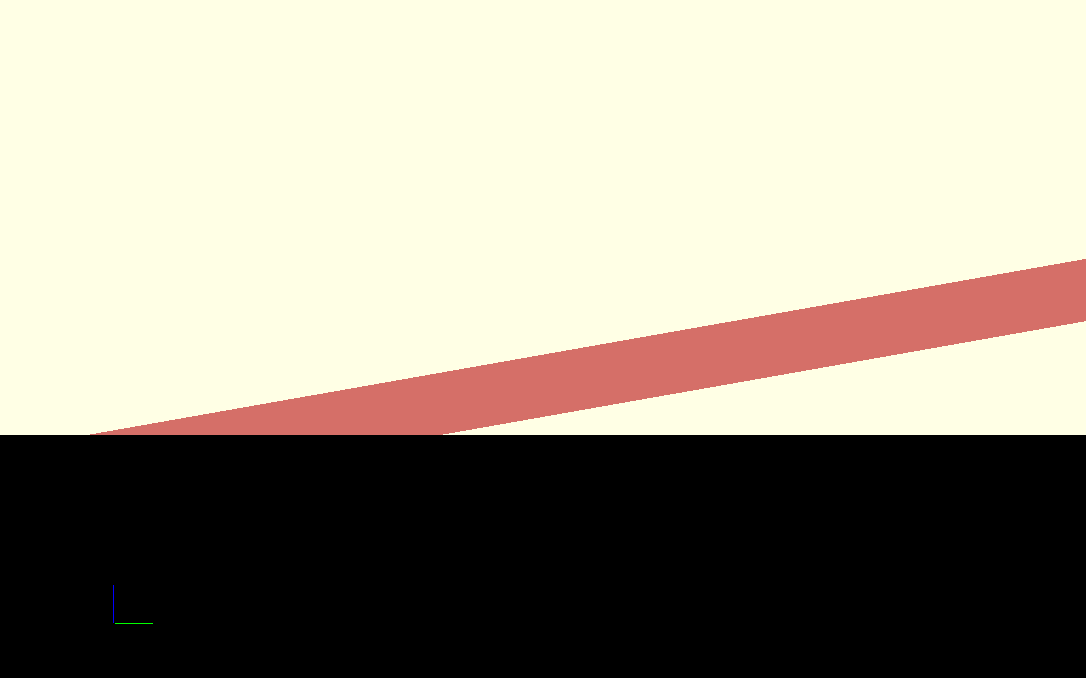
\includegraphics[width=.5\textwidth]{imagenes/otro-rayo-10}
    \caption[Sunbeam alternative  V]{Antonia's last attempt to dissuade Cecilia from using her alternate Sunbeam..}%\vspace{128in}
\label{fig:otro-rayo-10}
\end{figure}



Cecilia seemed to begin to understand.

---And with 10\si{\degree}? ---Antonia begged pointing to figure~\ref{fig:otro-rayo-10}.

---Clear! Cecilia gently tapped her forehead with one hand.
The spot of light on the floor begins to lengthen! 

What you need to measure is the intersection of the ray with the horizontal, not its cross section; that's why you drew the polygon the way you did.

---That's why I drew the polygon like this at the end--- Antonia underlined these last words. At first I did it like you. That's one of the reasons I like to write: it clarifies my ideas. Cecilia and Antonia looked at each other, smiling.

  

%%% Local Variables:
%%% mode: latex
%%% TeX-master: "../libro"
%%% End:
